\documentclass[12pt]{article}
%\renewcommand\normalsize{\fontsize{10pt}{12pt}\selectfont}
\usepackage{graphicx} % Required for inserting images
\usepackage[left=2cm,right=2cm,top=2cm,bottom=1.5cm]{geometry}
\usepackage{wrapfig}
%\pagestyle{empty} 

\title{HW 6}
%\author{Dennis Wilkinson}
%\date{March 31 2025; due Monday April 7}

\begin{document}

\setlength{\parindent}{0pt}
\setlength{\parskip}{3mm}

FS1 Wilkinson HW 6, due Thursday May 22

1. Charging by induction. It's possible to charge an object without touching it using induction. Here's one way:

a. An insulating (non-conducting) object is charged by friction, so it has a net positive charge (it gained electrons). Look up ``triboelectric series table" and list what materials could have been used to do this (rabbit fur?).

b. The positively charged insulator is brought near a neutral (no net charge, equal numbers of electrons and protons) metal sphere. Draw this and show what happens to the conduction electrons in the sphere. 

c. Now a metal wire is attached to the metal sphere and a very large conducting object (such as ``the ground" - Earth with some water and ions in it). Some of the conduction electrons from the ``ground" leave and go to sphere - why? Is the sphere neutral any more?

d. Finally, the wire is removed and then the insulating object moved away. Negative charge is left on the sphere. What would have happened if we had moved the object away before removing the wire?


\bigskip
\bigskip

2. Let's calculate the attractive force that would exist between the Earth and Sun if suddenly the electrons were all gone, leaving only protons. 

a. The Earth's mass is $6\times 10^{24}$ kg, and the sun's is $2\times 10^{30}$ kg. Figure out the average atomic mass (grams per mole) of the Earth and Sun (approximation okay, bonus for a really accurate calculation) and then roughly how many protons are in each. 

b. Now calculate the charge of only the protons in Earth and Sun, and then the Coulomb force that would exist between them if the electrons were gone. Compare to the actual gravitational force. 

c. (unrelated) In a lightning bolt, -50 C of charge is transferred from a cloud to the ground. How many moles of electrons is this?

\bigskip
\bigskip

3. Electric field lines.

\textbf{Important }- not mentioned in class - electric field lines point \textit{towards} negative charges, because a positive charge would feel a force towards a negative charge.

Go to https://phet.colorado.edu/en/simulations/charges-and-fields (search phet electric field) and run the simulator. You can place charges and it shows the electric field around them - experiment a bit to see how it works.


\begin{wrapfigure}[5]{l}{0.35\textwidth}
    \centering
    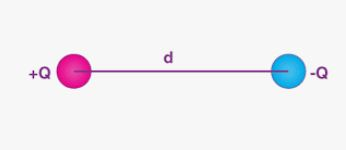
\includegraphics[width=\linewidth]{dipole.JPG}
\end{wrapfigure}
a. Draw a dipole, as below, and draw in the electric field lines around the charges. Try yourself and then use the tool to be sure your answer is right. You should draw in lines both next to, and far from, the charges. Field lines start on positive charges and end on negative charges, or at ``infinity" (far away).

b. Same question for this arrangement of charges:
\begin{figure}[h]
    \centering
    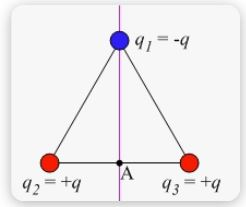
\includegraphics[width=0.3\linewidth]{charge triangle.JPG}
\end{figure}

c. Find the electric field - magnitude and direction - at point A in the drawing for part (b) if $q=30$ nC = $30 \times 10^{-9}$ C, the charges are equidistant, and the distance between $q_1$ and A is 2 cm. 

d. If a particle of charge -20 nC is placed at point A, find the magnitude and direction of the force on it. Once you know the electric field, force is easy - it's just $qE$. That's almost the definition of electric field, in some sense. 

e. Repeat parts (c) and (d) for point B, a distance 2 cm below point A. You need vectors now.

\bigskip
\bigskip

4a. Returning to the dipole from problem 3(a), set the origin of the coordinate system midway between the charges. Find an expression for the electric field - magnitude and direction - along the $x$ axis a distance $r$ from the origin, where $r>d/2$. Answer in terms of $k$, $Q$, $d$ and $r$. 

b. The dipole is a model for a polar molecule, such as NaCl or H$_2$O; this problem illustrates that $E$ fields far from such molecules are small. Use some values - your choice if atomic size or human size - for $Q$ and $d$ to calculate $E$ when $r=5d$, and when $r=100d$. Compare to the electric field if there was only the $+Q$ charge. 

c*. Return to you expression from part (a) and go to the limit of $r \gg d$. Use a Taylor expansion to find $E(r)$ to lowest order; compare the $r$ dependence to $E(r)$ for a point charge.

d*. Carbon dioxide is a linear molecule with the carbon in the middle. Its electrons spend a bit more time around the oxygen nuclei; we model this with a net negative charge of $-q$ on either O, and $2q$ on the C. Here $q$ is determined by quantum mechanics and is some fraction of the electron charge. Calculate $E$ along the axis of the CO$_2$ for some distance $r \gg d$, where $d$ is the distance between the nuclei. As for part (c), find the $r$ dependence in the $r \gg d$ limit. (This problem is touching on a ``multipole" expansion of an $E$ field - the CO$_2$ field only has the ``quadrupole" term, no dipole.)



\newpage


5. Let's model the bottom surface of a cloud as a flat sheet of negative charge. This charge induces an equal and opposite charge (positive) in the ground below. 

\begin{figure}[h]
    \centering
    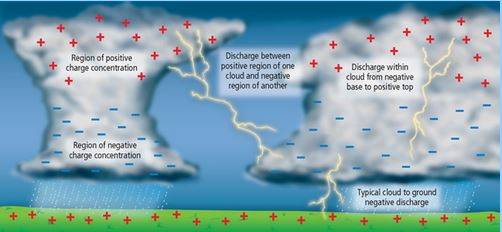
\includegraphics[width=0.7\linewidth]{lightning.JPG}
\end{figure}

a. The electric field between parallel sheets of charge is given by $E=\frac{Q}{\epsilon_0 A}$, where $Q$ is the charge on either sheet, and $A$ is their surface area. Amazingly, the field is constant and does not depend on the distance from the sheet - if we think of the sheet as infinite, that is. Try to think of a reason why this would be.

b. Say 100 C of charge has built up on the bottom of the cloud. Use a reasonable value/shape to find the cloud bottom's surface area (Rectangle? Circle? Maybe a km or so across?) and calculate $E$.

c. The air molecules will undergo \textit{dielectric breakdown} when $E>3 \times 10^6$ N/C. This means electrons will be l iberated from the atoms and can move freely, causing lightning. Will lightning strike for your numbers in part (a)?

d*. Let's derive $E=\frac{Q}{\epsilon_0 A}$. We have to assume the sheet is ``infinitely" large (the approximation is therefore valid when our distance from the sheet is small compared to the sheet's size, which may not be true for the cloud, but oh well). $Q$ is infinite, but so is $A$; instead, we define a finite charge density $\sigma=Q/A$. Clearly by symmetry, $E$ could only vary with the perpendicular distance to the sheet; let's call this distance $x$. 

To calculate $E$ at point $x$, the hard way, we have to add up the contributions from all the charge on the sheet. We consider a tiny area of the sheet $dA$ which has charge $\sigma dA$, and use $E=k\sigma dA/R^2$, where $R$ is the distance from $dA$ to the point in question.  Set up and perform this integral to find $E=\frac{Q}{2\epsilon_0 A}$; the $x$ dependence disappears here. (Since there is an equal and opposite second sheet in the cloud example, the answer for the cloud is twice this.) I recommend setting your origin directly ``under" $x$ and dividing the plane into rings of radius $r$; this reduces the integration to a single integral on $r$.

The easy way: Gauss' Law, if you've seen it or want to read about it. 
\end{document}